Graph theory is used widely and it is possible and desirable to implement graph traversals in parallel since graphs can be quite large.
This section does not describe graph theory in depth, but explains some basic notions of graphs and then describes how graph traversals can be implemented in parallel.

There are two types of graphs: undirected and directed graphs.
This section only considers undirected graphs.
An undirected graph \textit{G} is represented as a pair \textit{(V, E)}, where
\begin{itemizeSmall}
	\item[\textbf{V}], $V\notin \{\}$ and is called the set of vertices. A vertex can also be denoted as a "node".
	\item[\textbf{E}], set of unordered pairs of vertices and is called the set of edges.
	\item[\textbf{(u, v)}] is an edge which has two endpoints \textit{u} and \textit{v} where both are vertices.
\end{itemizeSmall}

A graph can be traversed and this means that each node of the graph is visited.
There are two types of graph traversals: breadth-first search, \textbf{BFS}, and depth-first search, \textbf{DFS}.
\begin{wrapfigure}{r}{0.3\textwidth}
	\begin{subfigure}[b]{0.3\textwidth}
		\begin{center}
			\fbox{
				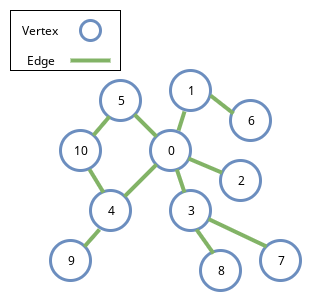
\includegraphics[width=1\textwidth]{figs/apps/bfs.png}
			}
		\end{center}
		\caption{Breadth-first traversal example}
		\label{fig:bfs}
	\end{subfigure}

		\begin{subfigure}[b]{0.3\textwidth}
		\begin{center}
			\fbox{
				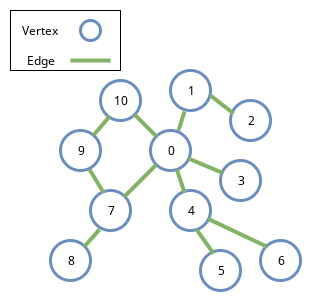
\includegraphics[width=1\textwidth]{figs/apps/dfs.png}
			}
		\end{center}
		\caption{Depth-first traversal example}
		\label{fig:dfs}
	\end{subfigure}

	\caption{Graph traversal examples}
\end{wrapfigure}
A breadth-first search traversal begins at a particular node and visits all neighboring nodes that are one hop away and labels them as they are visited. 
Then all nodes which have been visited one hop away from the starting point are now visiting all their one-hop-away neighbors. 
This is done iteratively until all nodes have been labeled and thus visited.
An example is seen in \autoref{fig:bfs}.

A depth-first search traversal begins at a particular node and picks a neighboring node which has not been visited yet. 
This node is then labeled as visited and yet another depth-first traversal is done from this node. 
If a node does not have an unvisited neighbor then it goes to a previously labeled node and picks an unlabeled neighboring node. 
This process is done iteratively until all nodes have been labeled as visited.
The process of a depth first traversal is shown in \autoref{fig:dfs}.

In general the \textit{DFS} is more memory efficient since it requires less state, but \textit{BFS} exposes more parallelism during the iterative traversal stages.
For this reason only \textit{BFS} is considered in parallel.

Explain the concept of a frontier in a graph.
Calculate distance from root (starting point) (min and max as functions of n)
Parallel algorithms to solve BFS.
Work complexity.
Code.
Optimizing runtime for graph traversal (lesson 6.2) very detailed and complex to describe in writing. Beware

Lesson 6.1